% Choose one to switch between slides and handout
\documentclass[]{beamer}
%\documentclass[handout]{beamer}

% Video Meta Data
\title{Bitcoin, Blockchain and Cryptoassets}
\subtitle{Alternative Consensus Protocols}
\author{Prof. Dr. Fabian Schär}
\institute{University of Basel}

% Config File
% Packages
\usepackage[utf8]{inputenc}
\usepackage{hyperref}
\usepackage{gitinfo2}
\usepackage{tikz}
\usepackage{amsmath}
\usepackage{bibentry}
\usepackage{xcolor}
\usepackage{colortbl} % Add colour to LaTeX tables
\usepackage{caption}
\usepackage[export]{adjustbox}
\usepackage{pgfplots} \pgfplotsset{compat = 1.17}

% Color Options
\definecolor{highlight}{rgb}{0.65,0.84,0.82}
\definecolor{focus}{rgb}{0.72, 0, 0}

% Beamer Template Options
\beamertemplatenavigationsymbolsempty
\setbeamertemplate{footline}[frame number]
\setbeamercolor{structure}{fg=black}
\setbeamercolor{footline}{fg=black}
\setbeamercolor{title}{fg=black}
\setbeamercolor{frametitle}{fg=black}
\setbeamercolor{item}{fg=black}
\setbeamercolor{}{fg=black}
\setbeamercolor{bibliography item}{fg=black}
\setbeamercolor*{bibliography entry title}{fg=black}
\setbeamertemplate{items}[square]
\setbeamertemplate{enumerate items}[default]
\captionsetup[figure]{labelfont={color=black},font={color=black}}
\captionsetup[table]{labelfont={color=black},font={color=black}}

\setbeamertemplate{bibliography item}{\insertbiblabel}

% Link Icon Command
\newcommand{\link}{%
    \tikz[x=1.2ex, y=1.2ex, baseline=-0.05ex]{%
        \begin{scope}[x=1ex, y=1ex]
            \clip (-0.1,-0.1)
                --++ (-0, 1.2)
                --++ (0.6, 0)
                --++ (0, -0.6)
                --++ (0.6, 0)
                --++ (0, -1);
            \path[draw,
                line width = 0.5,
                rounded corners=0.5]
                (0,0) rectangle (1,1);
        \end{scope}
        \path[draw, line width = 0.5] (0.5, 0.5)
            -- (1, 1);
        \path[draw, line width = 0.5] (0.6, 1)
            -- (1, 1) -- (1, 0.6);
        }
    }

% Read Git Data from Github Actions Workflow
% Defaults to gitinfo2 for local builds
\IfFileExists{gitInfo.txt}
	{\input{gitInfo.txt}}
	{
		\newcommand{\gitRelease}{(Local Release)}
		\newcommand{\gitSHA}{\gitHash}
		\newcommand{\gitDate}{\gitAuthorIsoDate}
	}

% Custom Titlepage
\defbeamertemplate*{title page}{customized}[1][]
{
  \vspace{-0cm}\hfill
\includegraphics[width=2.5cm]{../config/logo_cif}
  
\includegraphics[width=1.9cm]{../config/seal_wwz}
  \\ \vspace{2em}
  \usebeamerfont{title}\textbf{\inserttitle}\par
  \usebeamerfont{title}\usebeamercolor[fg]{title}\insertsubtitle\par  \vspace{1.5em}
  \small\usebeamerfont{author}\insertauthor\par
  \usebeamerfont{author}\insertinstitute\par \vspace{2em}
  \usebeamercolor[fg]{titlegraphic}\inserttitlegraphic
    \tiny \noindent \texttt{Release Ver.: \gitRelease}\\ 
    \texttt{Version Hash: \gitSHA}\\
    \texttt{Version Date: \gitDate}\\ \vspace{1em}
  \link \href{https://github.com/cifunibas/Bitcoin-Blockchain-Cryptoassets/blob/main/slides/intro.pdf}
  {Get most recent version}\\
  \link \href{https://github.com/cifunibas/Bitcoin-Blockchain-Cryptoassets/blob/main/slides/intro.pdf}
  {Watch video lecture}\\ \vspace{1em}
  License: \texttt{Creative Commons Attribution-NonCommercial-ShareAlike 4.0 International}\\\vspace{2em}
  
\includegraphics[width = 1.2cm]{../config/license}
}

% tikzlibraries
\usetikzlibrary{decorations.pathreplacing}
\usetikzlibrary{decorations.markings}
\usetikzlibrary{positioning}

%caption font
\captionsetup{font=footnotesize}

\usetikzlibrary{calc}

%%%%%%%%%%%%%%%%%%%%%%%%%%%%%%%%%%%%%%%%%%%%%%
%%%%%%%%%%%%%%%%%%%%%%%%%%%%%%%%%%%%%%%%%%%%%%
\begin{document}
	
	\thispagestyle{empty}
	\begin{frame}[noframenumbering]
		\titlepage
	\end{frame}
	
	
	%%%
	\begin{frame}{Why Consensus Matters}
		
		Distributed ledger as \color{focus} chain of transactions and states \color{black} whose \color{focus} compliance with an explicit rule set \color{black} is  attested by a reliable network of record keeping nodes.
		
		\uncover<2->{
			\vspace{1.5 em}
			\textbf{Account statement example:}
			
			\begin{center}
				\begin{tikzpicture}[scale=0.7, every node/.style ={scale=0.8}]
					
% Agent Savvy
	\node 			(savvy) at (12,0) {
\includegraphics[height = 2cm]{../assets/images/agents/handing_left.png}};
	\node			(as_official) at (10,0) {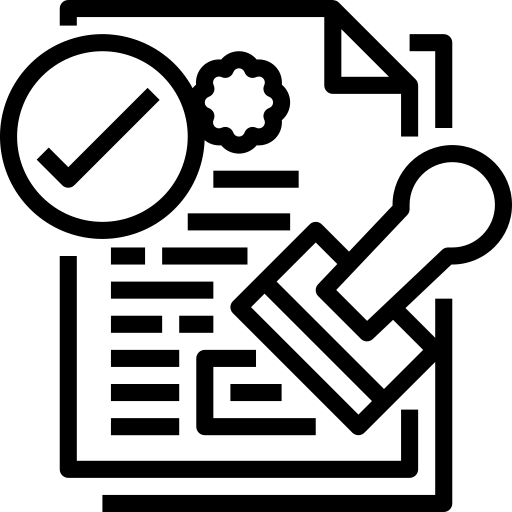
\includegraphics[height = 1.6 cm]{../assets/images/account_statement_official.png}};

% Agent Naive
	\node 			(naive) at (0,0) {
\includegraphics[height = 2 cm]{../assets/images/agents/handing_right.png}};
	\node			(as_DIY) at (2,0) {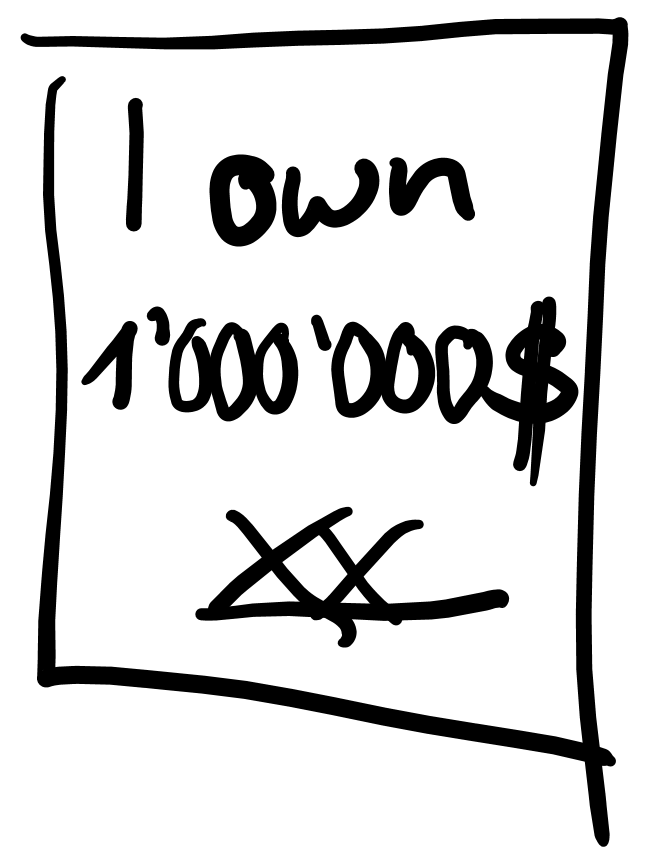
\includegraphics[height = 1.8cm]{../assets/images/account_statement_handmade.png}};

% Text
	
	\node  			at (6,0) {\LARGE vs.};

		

				\end{tikzpicture}
			\end{center}
			
			\vspace{1 em}
			
			$\Rightarrow$ Value of the ledger content relies on the network attesting it.
		}
		
	\end{frame}
	%%%	
	
	%%%
	\begin{frame}{Measures Supporting Consensus}
		
		\textbf{Explicit and unambiguous rule set} for legitimate changes to the ledger and block sequence.
		\vspace{0.25 em}
		
		$\Rightarrow$ Invalid blocks are detected easily and unambiguously.
		\vspace{1.5 em}
		
		\textbf{Decision mechanism} for consensus over different, legitimate extensions of the ledger. 
		\vspace{0.25 em}
		
		$\Rightarrow$ Swiftly resolving situations of uncertainty.
		\vspace{1.5 em}
		
		\textbf{Incentive system} that rewards compliant behaviour and / or penalizes manipulation attempts.
		\vspace{0.25 em}
		
		$\Rightarrow$ Typically in native protocol asset, tying the participant's interest to the sustainable value of the network.
		
	\end{frame}
	%%%
	
	%%%
	\begin{frame}{What Makes a Good Consensus Mechanism?}
		
		Suitability of a consensus mechanism \color{focus} depends on the purpose and user base \color {black} of a decentralized ledger.
		\vspace{1 em}
		
		\textbf{The Trilemma:}
		
		\begin{center}
			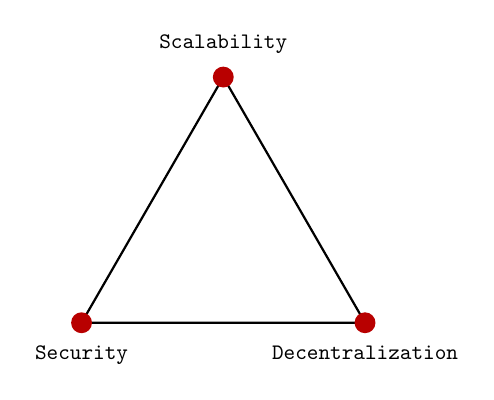
\begin{tikzpicture}[scale=0.6, every node/.style ={scale=0.8}]
				
% Title: Blockchain or Scalability Trilemma

% Arrangement
	\coordinate (A) at (0,0);
	\coordinate (B) at (3,5.2);
	\coordinate (C) at (6,0);


% Triangle
  \draw [thick]		 (A) -- (B) -- (C) -- (A);
  \node 			 at (A) [circle, fill = focus, minimum width=0.2cm,minimum height=0.2cm]{};
  	\node			 at	(A) [below = 0.2] {\texttt{Security}};
  \node 			 at (B) [circle, fill = focus, minimum width=0.2cm,minimum height=0.2cm]{};
  	\node			 at	(B) [above = 0.2] {\texttt{Scalability}};
  \node 			 at (C) [circle, fill = focus, minimum width=0.2cm,minimum height=0.2cm]{};
  	\node			 at	(C) [below = 0.2] {\texttt{Decentralization}};



			\end{tikzpicture}
		\end{center}
		
		\textbf{Generalized Rule:} Subject to tadeoffs, i.e., not possible to achieve all three goals. 	
	\end{frame}
	%%%	
	
	%%%
	\begin{frame}{Popular Consensus Mechanisms}
		We will look at and compare the following consensus mechanisms:
		
		\vspace{2.5em}
		
		\centering
		\begin{tikzpicture}[scale=1, every node/.style={scale=1}]
			\begin{footnotesize}
	\coordinate (1) at (-4, 3);
	\coordinate (2) at (0, 3);
	\coordinate (3) at (4, 3);
	
	\node (pow) at (1) {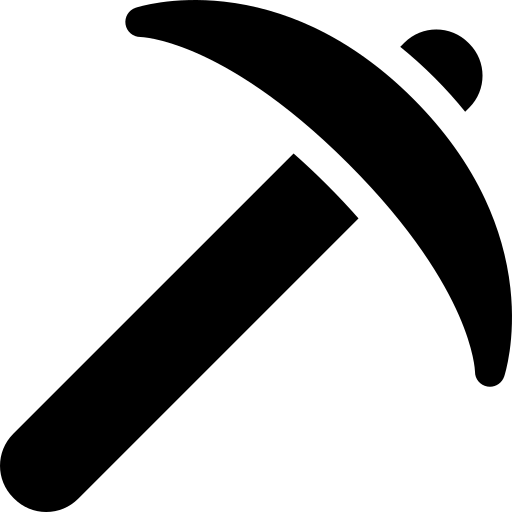
\includegraphics[height = 0.15\textheight]{../assets/images/pickaxe}};
	\node[below = 3pt] at (pow.south) {Proof of Work};
	
	\node (pos) at (2) {
\includegraphics[height = 0.15\textheight]{../assets/images/staking}};
	\node[below = 3pt] at (pos.south) {Proof of Stake};
	
	\node (poa) at (3) {
\includegraphics[height = 0.15\textheight]{../assets/images/bank}};
	\node[below = 3pt] at (poa.south) {Proof of Authority};
	
\end{footnotesize}

		\end{tikzpicture}
	\end{frame}
	%%%
	
	%%%
	\begin{frame}{Proof of Work Trilemma}
		\begin{center}
			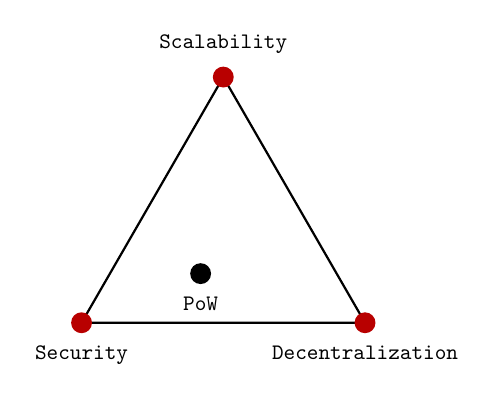
\begin{tikzpicture}[scale=0.6, every node/.style ={scale=0.8}]
				
% Title: Blockchain or Scalability Trilemma

% Arrangement
	\coordinate (A) at (0,0);
	\coordinate (B) at (3,5.2);
	\coordinate (C) at (6,0);


% Triangle
  \draw [thick]		 (A) -- (B) -- (C) -- (A);
  \node 			 at (A) [circle, fill = focus, minimum width=0.2cm,minimum height=0.2cm]{};
  	\node			 at	(A) [below = 0.2] {\texttt{Security}};
  \node 			 at (B) [circle, fill = focus, minimum width=0.2cm,minimum height=0.2cm]{};
  	\node			 at	(B) [above = 0.2] {\texttt{Scalability}};
  \node 			 at (C) [circle, fill = focus, minimum width=0.2cm,minimum height=0.2cm]{};
  	\node			 at	(C) [below = 0.2] {\texttt{Decentralization}};



				\coordinate (AC) at ($(A)!0.4!(C)$);
				\node (pow) at ($(AC)!0.2!(B)$) [circle, fill = black, minimum width=0.2cm,minimum height=0.2cm]{};
				\node at (pow) [below = 0.2] {\texttt{PoW}};
			\end{tikzpicture}
		\end{center}
	
		\begin{description}[labelwidth=10em]
			\item[\textbf{Scalability}] Every node needs to process every transaction. Block creation is very resource intensive.
			\item[\textbf{Decentralization}] Open network with many participants. Mining pools compromise decentralization.
			\item[\textbf{Security}] Secured by ressource allocation. Simplicity increases security.
		\end{description}
	\end{frame}
	%%%
	
	%%%
	\begin{frame}{Proof of Stake}
		To participate in the consensus network, each node - called a validator - needs to deposit and lock protocol base assets. This is called staking.
		
		\vspace{1.5 em}
		\textbf{Block creation and transaction validation:}
		Block creators are selected at random in proportion to their stake. A set of other validators will then attest to the validity of the created blocks.
		
		\vspace{1.5 em}
		\textbf{Malicious and unresponsive validators:}
		Malicious behaviour is punished by slashing (destroying a significant part) of the staked assets of the offenders. Failure to participate forfeits any rewards and might be punished furhter.
		
		\vspace{1.5 em}
		\textbf{Incentive system:}
		Validators receive returns on their stake by performing their duties. These rewards are funded by transaction costs and/or newly generated assets (inflation).
		
	\end{frame}
	%%%
	
	%%%
	\begin{frame}{Proof of Stake Trilemma}
		\begin{center}
			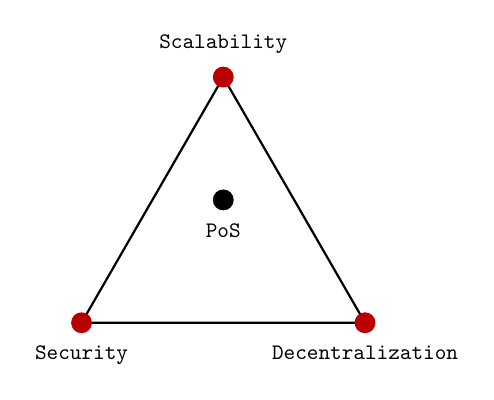
\begin{tikzpicture}[scale=0.6, every node/.style ={scale=0.8}]
				
% Title: Blockchain or Scalability Trilemma

% Arrangement
	\coordinate (A) at (0,0);
	\coordinate (B) at (3,5.2);
	\coordinate (C) at (6,0);


% Triangle
  \draw [thick]		 (A) -- (B) -- (C) -- (A);
  \node 			 at (A) [circle, fill = focus, minimum width=0.2cm,minimum height=0.2cm]{};
  	\node			 at	(A) [below = 0.2] {\texttt{Security}};
  \node 			 at (B) [circle, fill = focus, minimum width=0.2cm,minimum height=0.2cm]{};
  	\node			 at	(B) [above = 0.2] {\texttt{Scalability}};
  \node 			 at (C) [circle, fill = focus, minimum width=0.2cm,minimum height=0.2cm]{};
  	\node			 at	(C) [below = 0.2] {\texttt{Decentralization}};



				\coordinate (AC) at ($(A)!0.5!(C)$);
				\node (pos) at ($(AC)!0.5!(B)$) [circle, fill = black, minimum width=0.2cm,minimum height=0.2cm]{};
				\node at (pos) [below = 0.2] {\texttt{PoS}};
			\end{tikzpicture}
		\end{center}
		
		\begin{description}[labelwidth=10em]
			\item[\textbf{Scalability}] Only a set of validators need to process each transaction. Proposers are randomly selected.
			\item[\textbf{Decentralization}] Open network with many participants. Potential crowding out over time.
			\item[\textbf{Security}] Secured by staked capital. High complexity of the mechanism reduces security.
		\end{description}
	\end{frame}
	%%%
	
	%%%
	\begin{frame}{Proof of Authority}
		The consensus network consists of a \color{focus}small set of approved nodes\color{black} - called validators. These are often identified and have a reputation attached.
		
		\vspace{1.5 em}
		\textbf{Block creation and transaction validation:}
		Validators create and validate blocks. Other validators will attest to the validity of the created blocks.
		
		\vspace{1.5 em}
		\textbf{Malicious and unresponsive validators:}
		Malicious or unsresponsive behaviour is punished by excluding a validator and negatively impacting their reputation.
		
		\vspace{1.5 em}
		\textbf{Incentive system:}
		Block rewards are usually only the transaction costs.
		
	\end{frame}
	%%%
	
	%%%
	\begin{frame}{Proof of Authority Trilemma}
		\begin{center}
			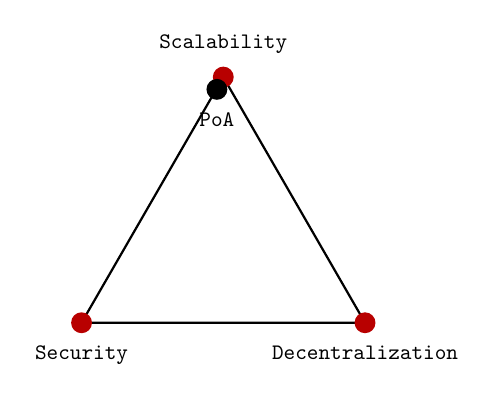
\begin{tikzpicture}[scale=0.6, every node/.style ={scale=0.8}]
				
% Title: Blockchain or Scalability Trilemma

% Arrangement
	\coordinate (A) at (0,0);
	\coordinate (B) at (3,5.2);
	\coordinate (C) at (6,0);


% Triangle
  \draw [thick]		 (A) -- (B) -- (C) -- (A);
  \node 			 at (A) [circle, fill = focus, minimum width=0.2cm,minimum height=0.2cm]{};
  	\node			 at	(A) [below = 0.2] {\texttt{Security}};
  \node 			 at (B) [circle, fill = focus, minimum width=0.2cm,minimum height=0.2cm]{};
  	\node			 at	(B) [above = 0.2] {\texttt{Scalability}};
  \node 			 at (C) [circle, fill = focus, minimum width=0.2cm,minimum height=0.2cm]{};
  	\node			 at	(C) [below = 0.2] {\texttt{Decentralization}};



				\coordinate (AC) at ($(A)!0.05!(C)$);
				\node (poa) at ($(AC)!0.95!(B)$) [circle, fill = black, minimum width=0.2cm,minimum height=0.2cm]{};
				\node at (poa) [below = 0.2] {\texttt{PoA}};
			\end{tikzpicture}
		\end{center}
		
		\begin{description}[labelwidth=10em]
			\item[\textbf{Scalability}] Very small set of validators and simple mechanism.
			\item[\textbf{Decentralization}] Closed network, validators can easily collude. Almost fully centralized.
			\item[\textbf{Security}] Simple mechanism and only approved validators provide a high security.
		\end{description}
	\end{frame}
	%%%
	
	%%%
	\begin{frame}{Consensus Trilemma}
		\begin{center}
			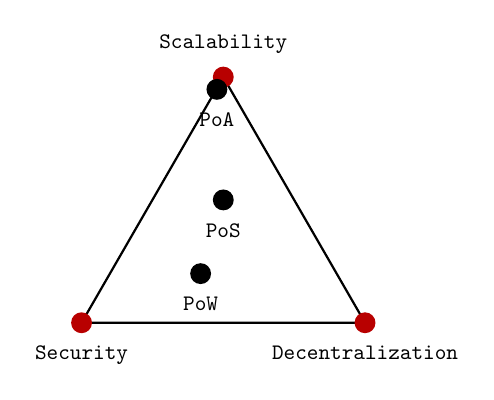
\begin{tikzpicture}[scale=0.6, every node/.style ={scale=0.8}]
				
% Title: Blockchain or Scalability Trilemma

% Arrangement
	\coordinate (A) at (0,0);
	\coordinate (B) at (3,5.2);
	\coordinate (C) at (6,0);


% Triangle
  \draw [thick]		 (A) -- (B) -- (C) -- (A);
  \node 			 at (A) [circle, fill = focus, minimum width=0.2cm,minimum height=0.2cm]{};
  	\node			 at	(A) [below = 0.2] {\texttt{Security}};
  \node 			 at (B) [circle, fill = focus, minimum width=0.2cm,minimum height=0.2cm]{};
  	\node			 at	(B) [above = 0.2] {\texttt{Scalability}};
  \node 			 at (C) [circle, fill = focus, minimum width=0.2cm,minimum height=0.2cm]{};
  	\node			 at	(C) [below = 0.2] {\texttt{Decentralization}};



				
				\coordinate (AC) at ($(A)!0.4!(C)$);
				\node (pow) at ($(AC)!0.2!(B)$) [circle, fill = black, minimum width=0.2cm,minimum height=0.2cm]{};
				\node at (pow) [below = 0.2] {\texttt{PoW}};
				
				\coordinate (AC) at ($(A)!0.5!(C)$);
				\node (pos) at ($(AC)!0.5!(B)$) [circle, fill = black, minimum width=0.2cm,minimum height=0.2cm]{};
				\node at (pos) [below = 0.2] {\texttt{PoS}};
				
				\coordinate (AC) at ($(A)!0.05!(C)$);
				\node (poa) at ($(AC)!0.95!(B)$) [circle, fill = black, minimum width=0.2cm,minimum height=0.2cm]{};
				\node at (poa) [below = 0.2] {\texttt{PoA}};
			\end{tikzpicture}
		\end{center}
		
		\textbf{Conclusion:} All mechanisms have tradeoffs and might be suited for different use cases.
	\end{frame}
	%%%
	
	
%	\begin{frame}%[allowframebreaks]
%		\frametitle{References}
%		\bibliographystyle{amsplain}
%		\bibliography{../assets/bib/refs}
%	\end{frame}
	
\end{document}